\section{Identifying Metamorphic Relations} 
We identified seven metamorphic properties for each dataset used: rotation, shearing, shading, shifting along x-axis, shifting along-axis, zooming along x-axis, zooming along y-axis. Each image in the testing dataset (digit, letter, and, fashion) was transformed using the seven metamorphic properties. We used Keras image preprocessing functions to apply these transformations to the test data in each dataset to generate new data to measure robustness.
\subsection{Rotate}
The test images from each dataset is transformed The rotation transformation algorithm takes in an image and an angle in degrees as parameter and rotates the image with the given angle. For each angle in [\ang{-50}, \ang{50}] we transformed each image Each image (digit, letter, and, fashion) is rotated clockwise and counter clockwise between angles [\ang{-50}, \ang{50}]. 
    \begin{figure}[!htbp]
        \centering
        \begin{subfigure}[b]{.3\textwidth}
            \centering
            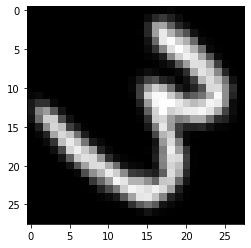
\includegraphics[width=\linewidth]{images/rotate1.png}
            \caption{Angle: \ang{-50}}
            \label{fig:Rotate-misclass0}
        \end{subfigure}%
        \begin{subfigure}[b]{.3\textwidth}
            \centering
            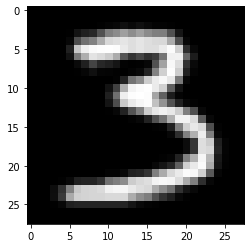
\includegraphics[width=\textwidth]{images/rotate2.png}
            \caption{Angle: \ang{0}}
            \label{fig:Rotate-misclass0}
        \end{subfigure}%
        \begin{subfigure}[b]{.3\textwidth}
            \centering
            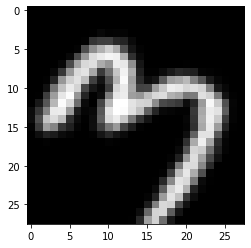
\includegraphics[width=\linewidth]{images/rotate3.png}
            \caption{Angle: \ang{50}}
            \label{fig:Rotate-misclass0}
        \end{subfigure}
        \caption{Rotation property applied to Digit 3.}
        \label{fig:Rotate-misclassifications}
    \end{figure}
    \FloatBarrier

\subsection{Shear}  
    \begin{figure}[!htbp]
        \centering
        \begin{subfigure}[b]{.3\textwidth}
            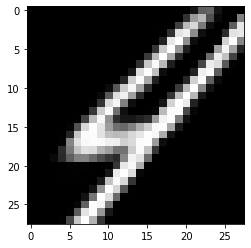
\includegraphics[width=\linewidth]{images/shear1.png}
            \caption{Angle: \ang{-50}}
            \label{fig:Rotate-misclass0}
        \end{subfigure}%
        \begin{subfigure}[b]{.3\textwidth}
            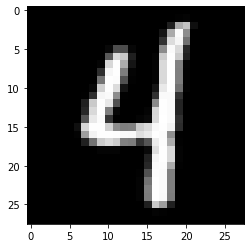
\includegraphics[width=\textwidth]{images/shear2.png}
            \caption{Angle: \ang{-50}}
            \label{fig:Rotate-misclass0}
        \end{subfigure}%
        \begin{subfigure}[b]{.3\textwidth}
            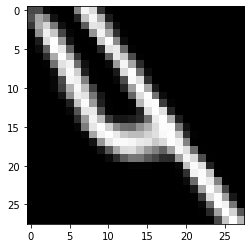
\includegraphics[width=\linewidth]{images/shear3.png}
            \caption{Angle: \ang{-50}}
            \label{fig:Rotate-misclass0}
        \end{subfigure}
        
        \caption{Shear property applied to Digit 4.}
        \label{fig:Rotate-misclassifications}
    \end{figure}
    \FloatBarrier
    
\subsection{Shading}
    \begin{figure}[htb!]
        \centering
        \begin{subfigure}[b]{.3\textwidth}
            \centering
            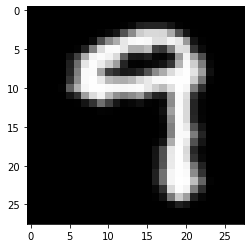
\includegraphics[width=\linewidth]{images/shade1.png}
            \caption{Value: 0}
            \label{fig:Rotate-misclass0}
        \end{subfigure}%
        \begin{subfigure}[b]{.3\textwidth}
            \centering
            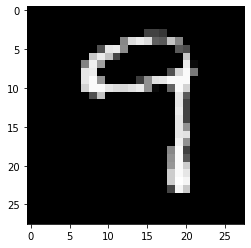
\includegraphics[width=\textwidth]{images/shade2.png}
            \caption{Value: 80}
            \label{fig:Rotate-misclass0}
        \end{subfigure}%
        \begin{subfigure}[b]{.3\textwidth}
            \centering
            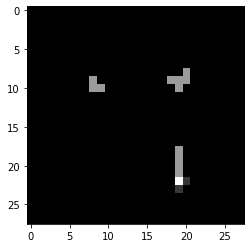
\includegraphics[width=\linewidth]{images/shade3.png}
            \caption{Value: 99}
            \label{fig:Rotate-misclass0}
        \end{subfigure}
        
        \caption{Shade property applied to Digit 9.}
        \label{fig:Rotate-misclassifications}
    \end{figure}
    \FloatBarrier
    
\subsection{Shifting in the X direction}
    For any value above x the image was completely out of the frame.
    \begin{figure}[htb!]
        \centering
        \begin{subfigure}[b]{.3\textwidth}
            \centering
            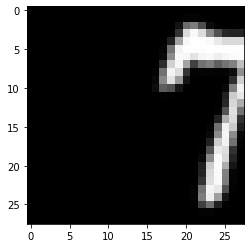
\includegraphics[width=\linewidth]{images/shiftx1.png}
            \caption{Value: -10}
            \label{fig:Rotate-misclass0}
        \end{subfigure}%
        \begin{subfigure}[b]{.3\textwidth}
            \centering
            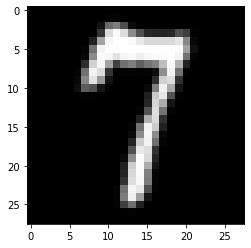
\includegraphics[width=\textwidth]{images/shiftx2.png}
            \caption{Value: 0}
            \label{fig:Rotate-misclass0}
        \end{subfigure}%
        \begin{subfigure}[b]{.3\textwidth}
            \centering
            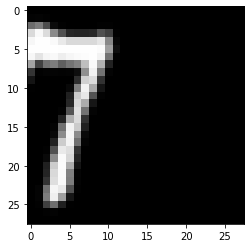
\includegraphics[width=\linewidth]{images/shiftx3.png}
            \caption{Value: 10}
            \label{fig:Rotate-misclass0}
        \end{subfigure}
        
        \caption{Shift X property applied to Digit 7.}
        \label{fig:Rotate-misclassifications}
    \end{figure}
    \FloatBarrier
    
\subsection{Shifting in the Y direction}
    \begin{figure}[htb!]
        \centering
        \begin{subfigure}[b]{.3\textwidth}
            \centering
            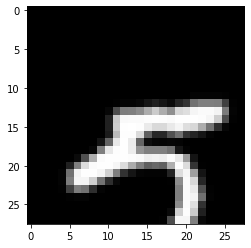
\includegraphics[width=\linewidth]{images/shifty1.png}
            \caption{Value: -10}
            \label{fig:Rotate-misclass0}
        \end{subfigure}%
        \begin{subfigure}[b]{.3\textwidth}
            \centering
            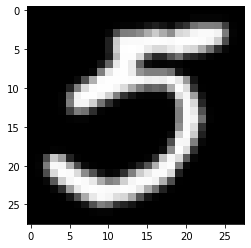
\includegraphics[width=\textwidth]{images/shifty2.png}
            \caption{Value: 0}
            \label{fig:Rotate-misclass0}
        \end{subfigure}%
        \begin{subfigure}[b]{.3\textwidth}
            \centering
            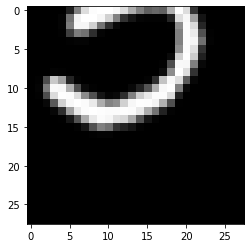
\includegraphics[width=\linewidth]{images/shifty3.png}
            \caption{Value: 10}
            \label{fig:Rotate-misclass0}
        \end{subfigure}
        
        \caption{Shift Y property applied to Digit 5.}
        \label{fig:Rotate-misclassifications}
    \end{figure}
    \FloatBarrier
